\documentclass{beamer}

\usepackage[spanish]{babel}
\usepackage[utf8]{inputenc}
\usepackage[T1]{fontenc}
\usepackage{amsmath,amssymb,amsfonts}
\usepackage{xcolor}
\usepackage{ragged2e}
\usepackage{etoolbox}
\usepackage{lipsum}
\usepackage{csquotes}
\usepackage[center]{caption}
\usepackage[export]{adjustbox}
\usepackage{biblatex}
\graphicspath{{../Imágenes}}

\addbibresource{biblio.bib}

\usetheme{Madrid}
\title[Ecuaciones Integrales]{Resolución numérica de ecuaciones Integrales} 
\author[Alfonso y Luis]{Alfonso de Lucas Iniesta y Luis Lucas García}
\institute[UA]{Universidad de Alicante - Facultad de Ciencias - Grado en física}
\date{Diciembre de 2024}

\apptocmd{\frame}{}{\justifying}{}
\addtobeamertemplate{block begin}{}{\justifying} % Justify all blocks

\begin{document}

\maketitle

\begin{frame}{Índice}
    \tableofcontents
\end{frame}

\begin{frame}{Introducción}
    \section{Introducción}
    Función desconocida $y(x)$.
    \begin{block}{Definiciones \cite{navarro2011ecuaciones}}
        Ecuación de Fredholm primera especie,
        \begin{equation}
            f(x)= \int_a^b K(x, s) y(s) \, ds
        \end{equation}
        Ecuación de Fredholm de segunda especie,
        \begin{equation}
            y(x)= f(x)+\lambda\int_a^b K(x, s) y(s) \, ds
        \end{equation}
    \end{block}  
\end{frame}

\begin{frame}{Introducción}
    \begin{block}{Definiciones}
         Ecuación de Volterra de primera especie,
        \begin{equation}
            f(x)= \int_a^x K(x, s) y(s) \, ds
        \end{equation}
        Ecuación de Volterra de segunda especie,
        \begin{equation}
             y(x)= f(x)+\int_a^x K(x, s) y(s) \, ds
             \label{Volterra 2es}
        \end{equation}
    \end{block}
    En todos los casos, $y(x)$ es la función desconocida. $K(x,s)$ es denotado como el \textbf{núcleo} y $f(x)$ se presume conocida.
    Cuando $f(x)= 0$ decimos que la ecuación integral es \textbf{homogénea}.
\end{frame}

\begin{frame}{Motivación}
    \section{Motivación}
    ¿Por qué razones querríamos nosotros estudiar las ecuaciones integrales?
    \begin{itemize}
        \item Condiciones de contorno particulares 
        \item Más ventajosa y elegante en la resolución de ciertos problemas
        \item Resolución de problemas específicos
    \end{itemize}
    \begin{figure}
        \centering
        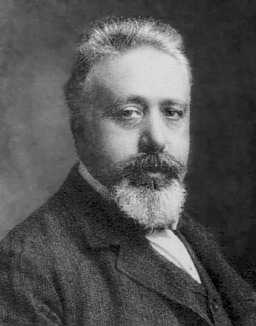
\includegraphics[width=0.25\linewidth]{Volterra.png}
        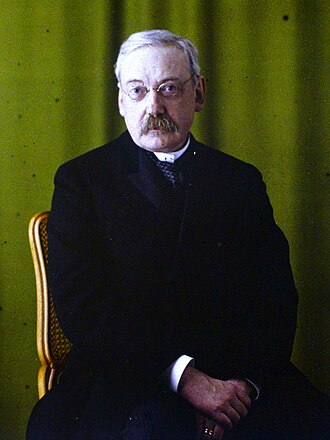
\includegraphics[width=0.24\linewidth]{Fredholm.png}
        \caption{Los matemáticos Vito Volterra a la izquierda y Erik Ivar Fredholm a la derecha}
        \label{fig:enter-label}
    \end{figure}  
\end{frame}

\begin{frame}{Método del rectángulo \cite{10.1093/comjnl/12.4.393}}\section{Resolución de Volterra}
    Tomando una escuación de Volterra de segunda especie cualquiera (\ref{Volterra 2es}). Vamos a utilizar la regla de aproximación más simple. Si queremos la solución en un intervalo $[0, T]$, podemos separar este intervalo en N subintervalos con forma $\Delta s = \frac{T}{N}$ y $t_n = n \frac{T}{N}$, con $n=0, 1, \ldots, N$.
    \begin{block}{Regla del rectángulo}
        Tomando una primera aproximación sencilla de la integral (base por altura), tomando el valor de $k(t, s)$ al inicio del intervalo, se tiene que:
        \begin{equation}
            y(t_n) = g(t_n) + n\frac{T}{N} \sum_{i=0}^{n-1} k(t_n, t_i) y(t_i)
        \end{equation}
    \end{block}
    Esta expresión nos resulta familiar, y es que podemos expresar este problema en forma de matriz. Si lo escribimos en índices:
    $$
    y_n = g_n + \frac{T}{N} \sum_{i=0}^{n-1} k_n^i y^i
    $$
\end{frame}

\begin{frame}{Otros métodos de la integral}
    \begin{block}{Regla del trapecio}
        Si tomamos una aproximación algo más complicada para la integral en la ecuación, obtendríamos que queda:
        \begin{equation}
            y(t_n) = g(t_n) + \frac{T}{2N}\sum_{i=0}^{n-1} \left(k(t_n, t_i)y(t_i) + k(t_n, t_{i+1})y(t_{i+1})\right)
        \end{equation}
    \end{block}
    \begin{figure}[h!]
        \centering
        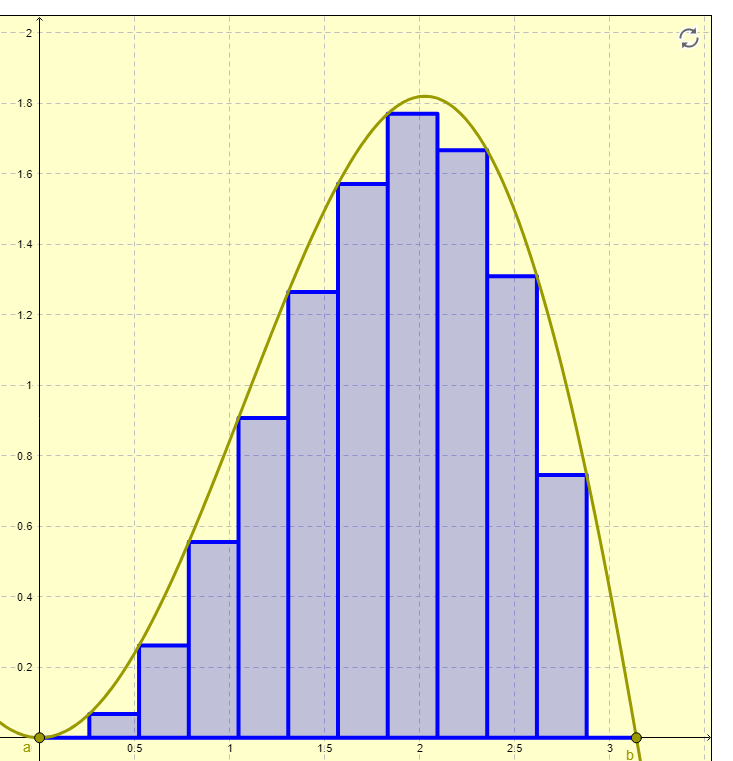
\includegraphics[max width=0.25\linewidth]{SumaRect}
        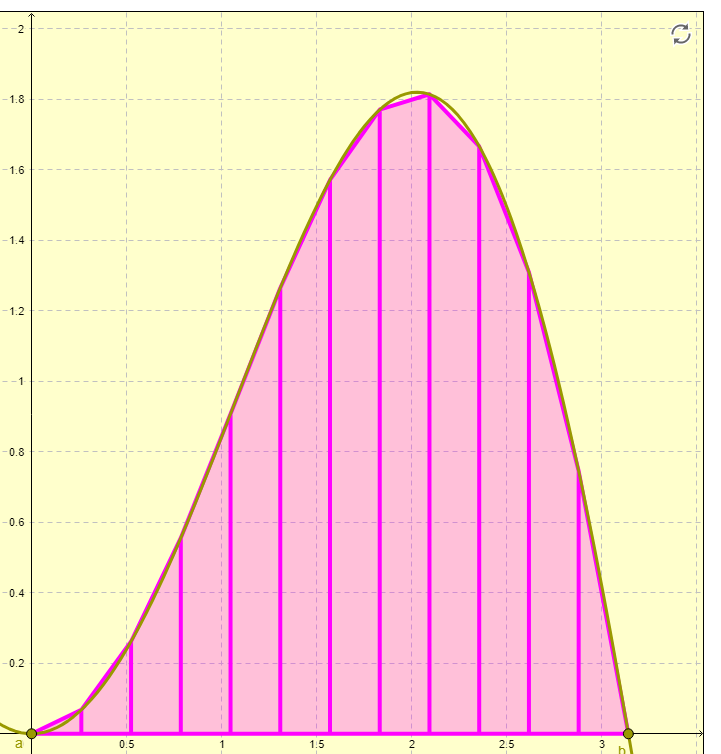
\includegraphics[max width=0.25\linewidth]{SumaTrap}
        \caption{Reglas de integración numérica del rectángulo y el trapecio.}
        \label{fig:reglasTrapSum}
    \end{figure}
\end{frame}

\begin{frame}{Resolución de un caso particular \cite{WolframAlphaVolt}}
    \begin{figure}
        \centering
        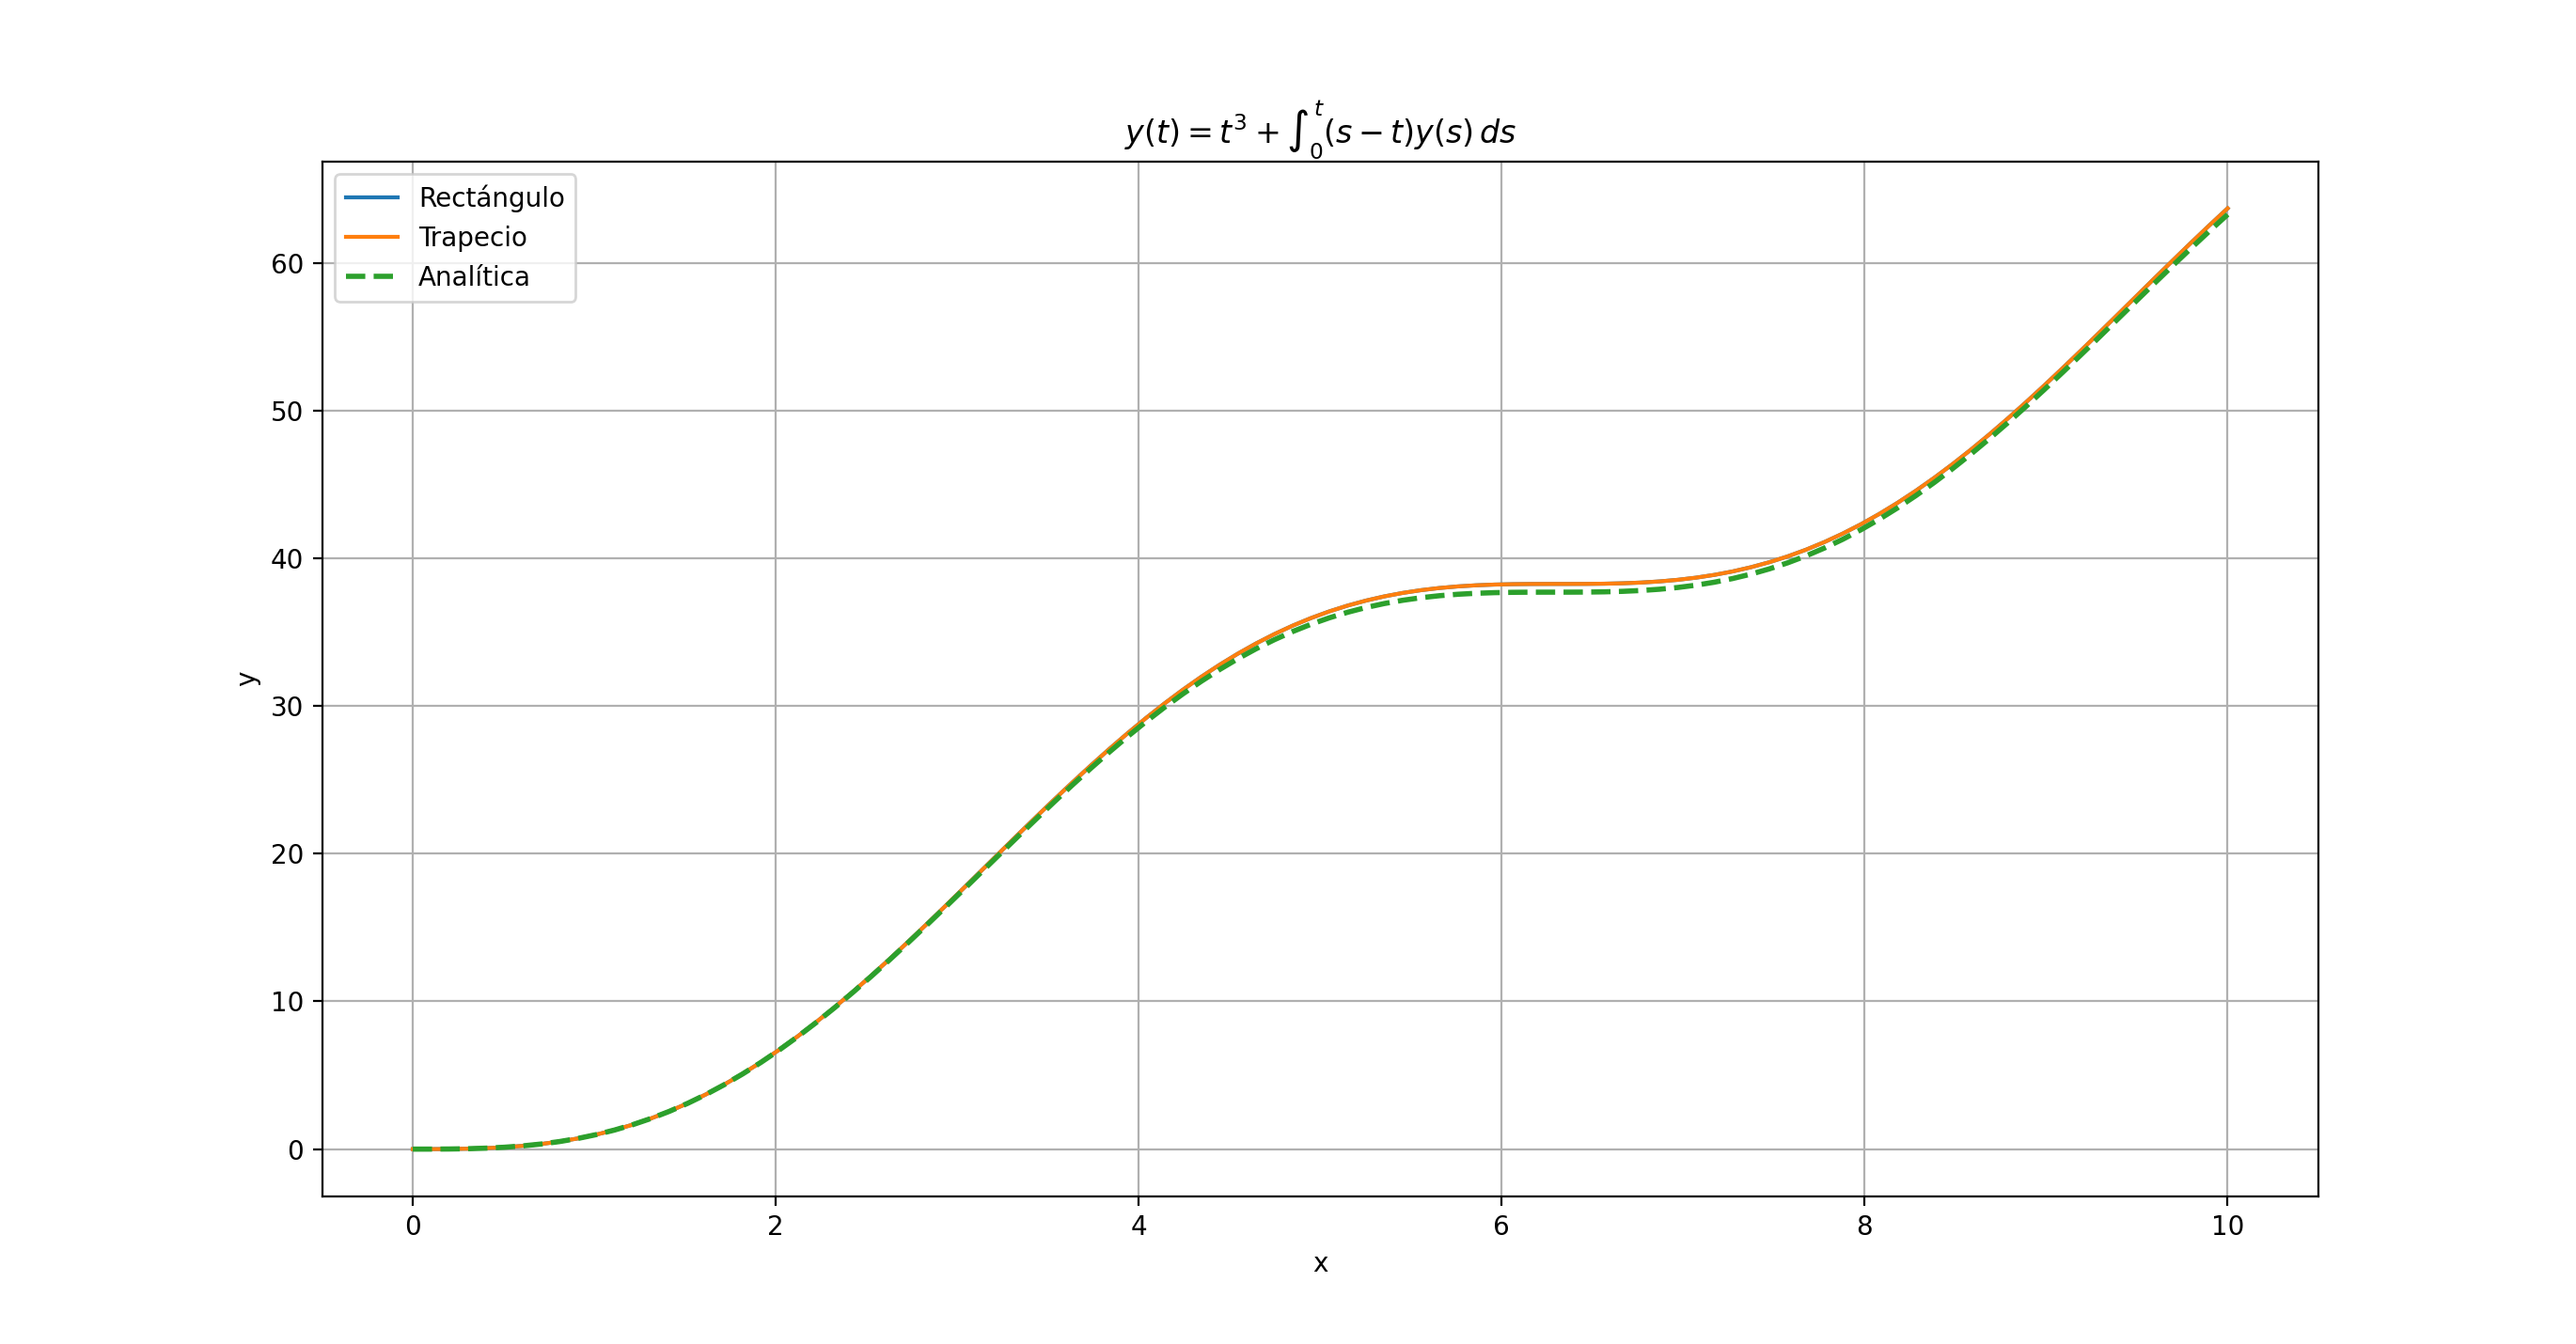
\includegraphics[max width=\linewidth]{VolterraSol}
        \caption{Solución de un problema de la referencia \cite{navarro2011ecuaciones}}
        \label{fig:SolucionVolt}
    \end{figure}
\end{frame}
\begin{frame}{Análisis de ambos métodos}
    \begin{figure}
        \centering
        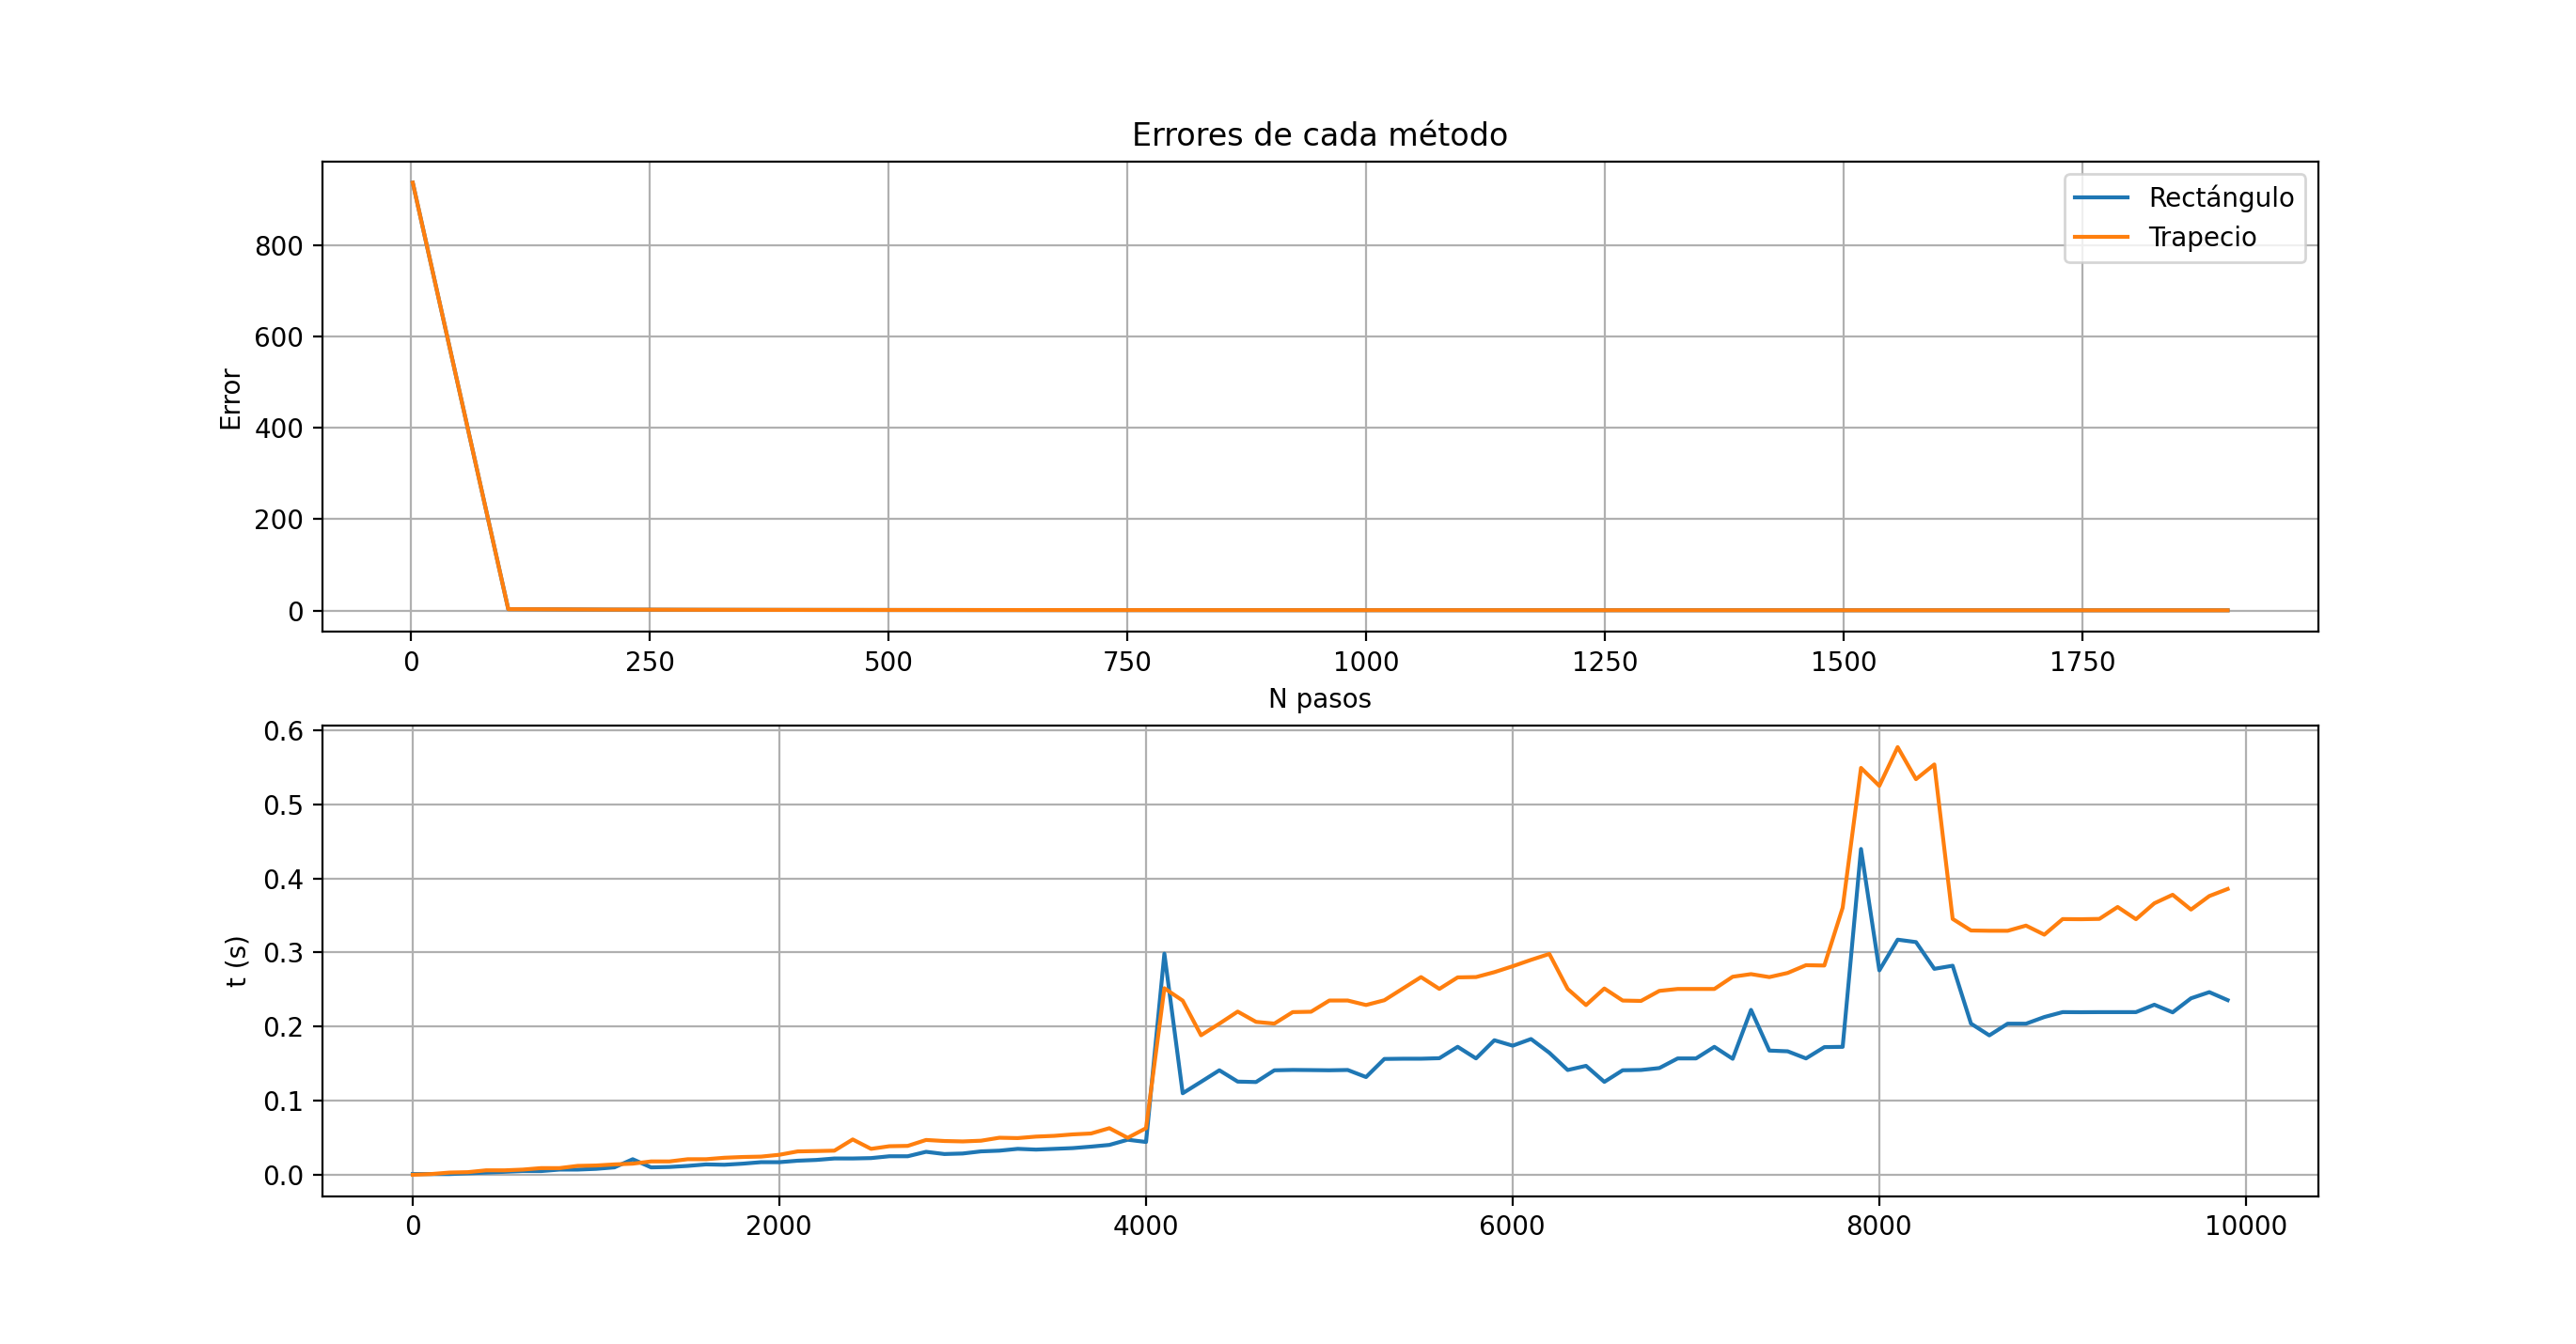
\includegraphics[max width=\linewidth]{VolterraErrs}
        \caption{Error y tiempo de ejecución para cada uno de los métodos de resolución de la figura \ref{fig:SolucionVolt}}
        \label{fig:volterraAnal}
    \end{figure}
\end{frame}

\begin{frame}{Oscilaciones libres en una cuerda \cite{rahman2007integral}}
    \section{Oscilaciones libres en una cuerda}
    \begin{figure}
        \centering
        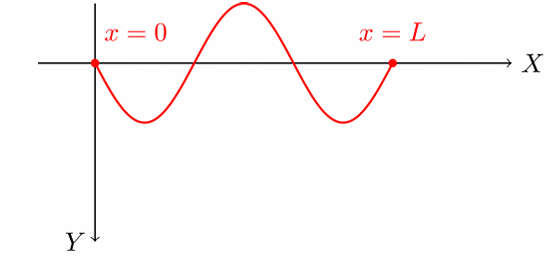
\includegraphics[width=1\linewidth]{Cuerda.png}
        \caption{Nuestra cuerda}
        \label{fig:enter-label}
\end{figure}
    
\end{frame}
\begin{frame}{Oscilaciones libres en una Cuerda}
    Sea $y(x,t)$ la posición en el instante $t$ de un punto de la cuerda con abcisa $x$. Sea $\lambda$ la densidad lineal de la cuerda, supuesta constante por simplicidad.
    \begin{block}{Fuerza de Inercia}
        Siguiendo la 2ª Ley de Newton, la fuerza de inercia de la cuerda por unidad de longitud viene dada por:
        \begin{equation}
            -\lambda\frac{\partial^2y(\xi,t)}{\partial t^2}
        \end{equation}
    \end{block}
    Donde el signo menos proviene de que la fuerza de inercia se opone a las oscilaciones de la cuerda.   
\end{frame}

\begin{frame}{Oscilaciones libres en una Cuerda}
    De esta manera la expresión va a tomar la forma siguiente:
    \begin{block}{Forma de la ecuación}
        \begin{equation}
           y(x,t)= -\lambda \int^L_0 K(x,\xi)\frac{\partial^2y(\xi,t)}{\partial t^2} d\xi
        \end{equation}
        Si consideramos que la cuerda realiza oscilaciones armónicas, es decir, $y(x,t)= y(x)sen(wt)$, donde $w>0$ es la frecuencia (fija) e $y(x)$ es la amplitud de las socilaciones resulta que:

        \begin{equation}
            y(x,t)= \lambda w^2\int^L_0 K(x,\xi)y(\xi)sen(wt) d\xi
            \label{ya casi está}
        \end{equation}
        Donde:
        $$
        K(x, \xi) = \left\{ \begin{array}{c}
        \frac{x(L-\xi)}{T_0 L}, \, 0 \leq x \leq \xi \\
        \frac{(L-x)\xi}{T_0 L}, \, \xi \leq x \leq L      
        \end{array} \right.
        $$
    \end{block}
\end{frame}

\begin{frame}{Oscilaciones libres en una Cuerda}
    Para finalizar, recordando que $y(x,t)= y(x)sen(wt)$ y diviendo por $sen(wt)$ a ambos lados de (\ref{ya casi está}) tenemos que:
    \begin{block}{Forma de la ecuación}
        \begin{equation}
            y(x)= \lambda w^2\int^L_0 K(x,\xi)y(\xi) d\xi
        \end{equation}
    \end{block}
    La cual es la expresión de una ecuación de Fredholm de segunda especie, en este caso homogénea.
\end{frame}

\begin{frame}{Resolución numérica de las Oscilaciones}
    Nuevamente emplearemos la regla del rectángulo y del trapecio, de forma que, en este caso la expresión queda de la siguiente manera.
    \begin{block}{Rectángulo y trapecio}
        Rectángulo:
        \begin{equation}
            y_n = g_n + \frac{T}{N} \sum_{i=0}^{N-1} k_n^i y^i
        \end{equation}
        Trapecio:
        \begin{equation}
            y(t_n) = g(t_n) + \frac{T}{2N}\sum_{i=0}^{N-1} \left(k(t_n, t_i)y(t_i) + k(t_n, t_{i+1})y(t_{i+1})\right)
        \end{equation}
    \end{block}
    
\end{frame}

\begin{frame}{Armónicos de la cuerda}
\begin{figure}
    \centering
    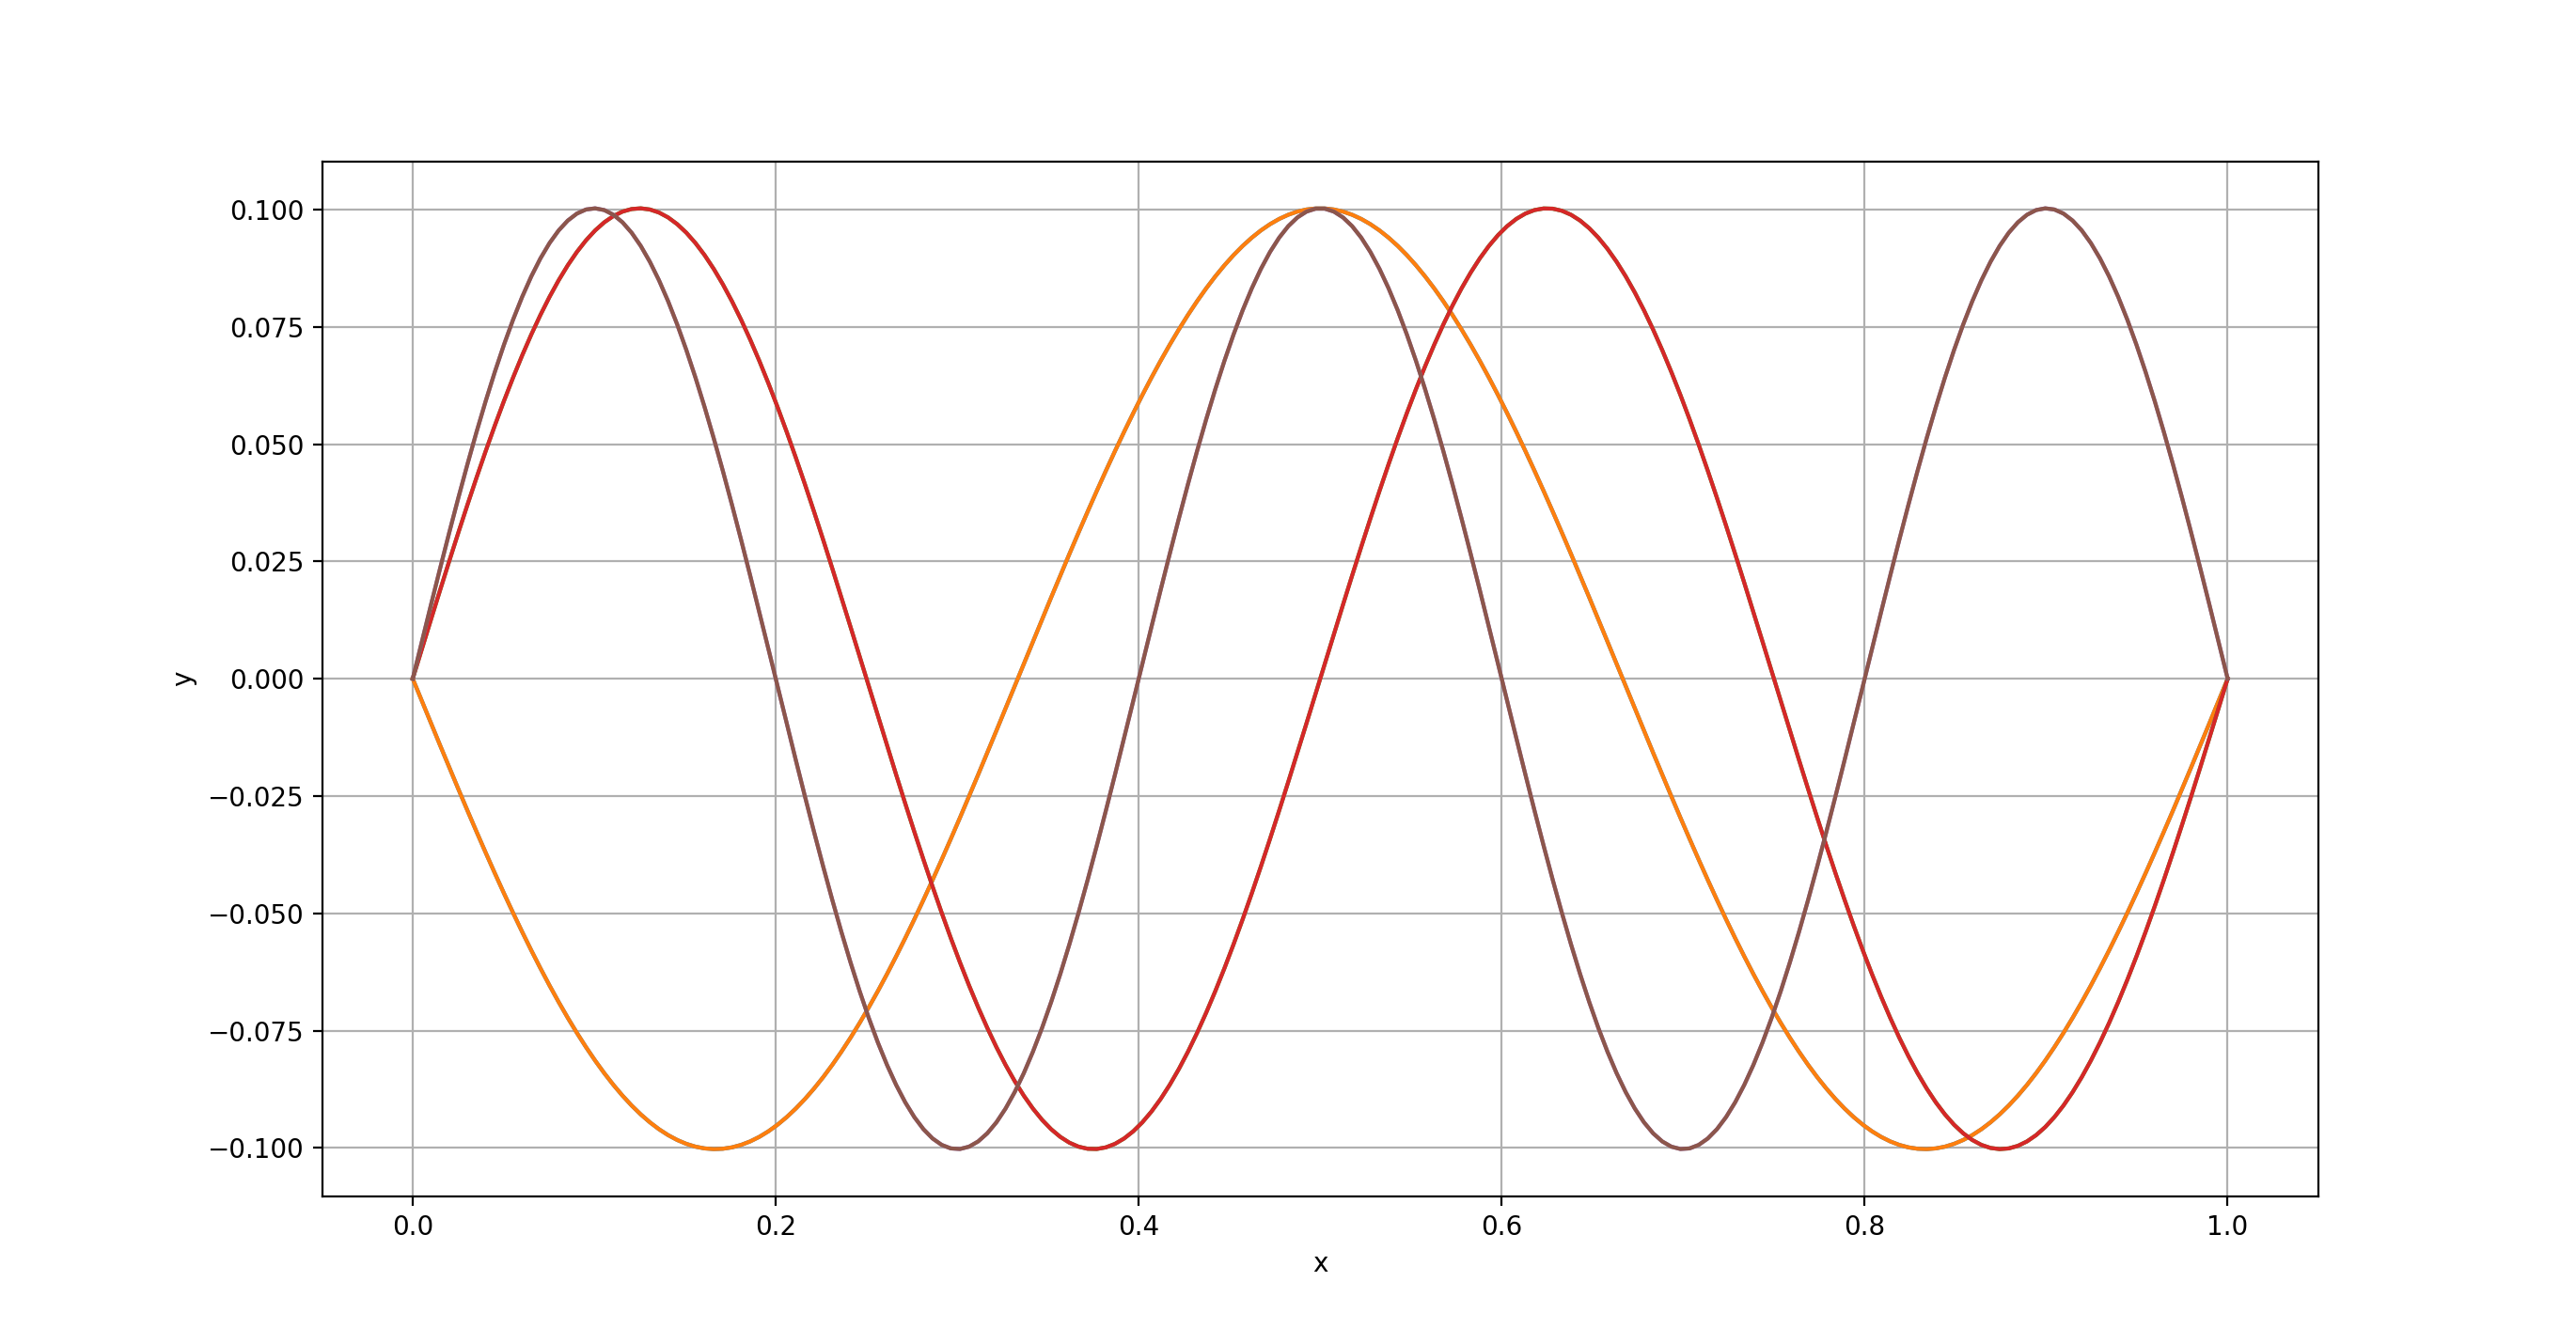
\includegraphics[max width=\linewidth]{FredholmArm}
    \caption{Oscilaciones de la cuerda con extremos fijos. Resolviendo la ecuación integral.}
    \label{fig:enter-label}
\end{figure}
\end{frame}

\begin{frame}{Conclusiones y Aplicaciones}\section{Conlusiones y Aplicaciones}

    \begin{itemize}
        \item Herramienta rápida y elegante 
        \item Procesos de coagulación
        \item Dinámica pobalcional
        \item Estabilidad de reactores nucleares
        \item Teoría de fotoesferas en Astrofísica \cite{sobolev1969course}
    \end{itemize}
    \begin{figure}
        \centering
        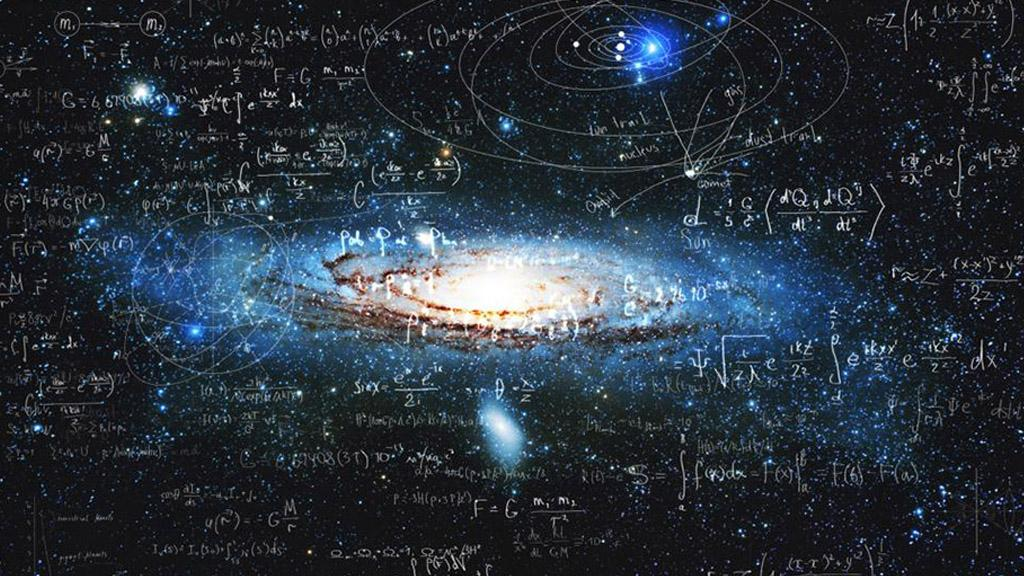
\includegraphics[width=0.5\linewidth]{fotosfera.png}
        \label{fig:enter-label}
    \end{figure}
    
\end{frame}

\begin{frame}[allowframebreaks]{Bibliografía}
    \section{Bibliografía}
    \printbibliography
\end{frame}

\end{document}
